\section{Reducción de la complejidad ciclomática}

	\subsection{Estado del proyecto antes de las correcciones}

		\paragraph{}Antes de empezar de trabajar en esta práctica, comprobaremos cuál es el estado del proyecto antes de empezar a trabajar. Para ello, ejecutaremos los test de cppcheck y metriculator. En las siguientes capturas de pantalla observamos los resultados arrojados.

 		\begin{figure}[H]
 			\centering
 			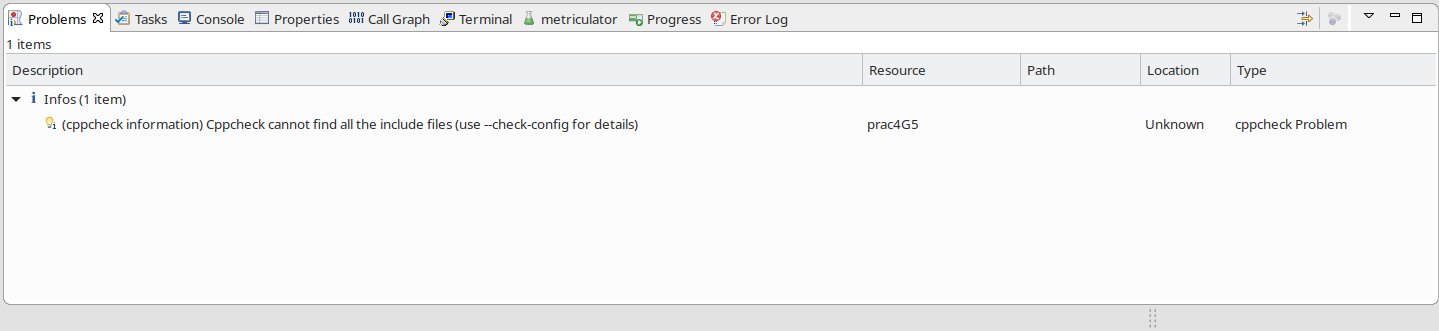
\includegraphics[scale=0.32]{img/captura94.png}
 			\caption{Captura de pantalla de los resultados arrojados tras la ejecución de cppcheck.}
 			\label{captura94}
 		\end{figure}
 	
 		\begin{figure}[H]
 			\centering
 			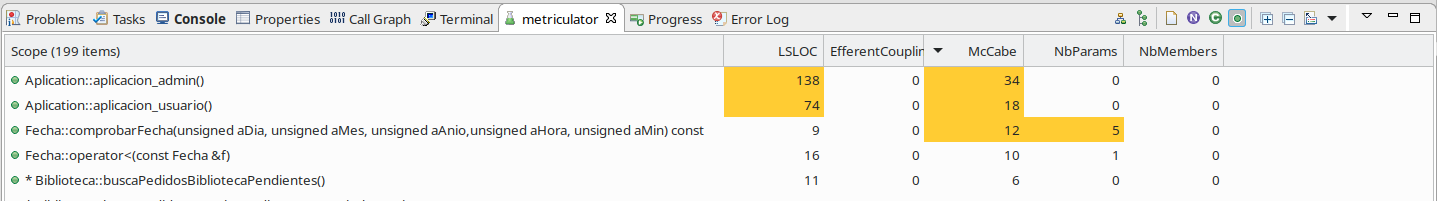
\includegraphics[scale=0.32]{img/captura95.png}
 			\caption{Captura de pantalla de los resultados arrojados tras la ejecución de metriculator.}
 			\label{captura95}
 		\end{figure}
 	
 		\paragraph{}En los resultados arrojados por cppcheck, podemos observar que tenemos un info: no se encuentran todos los includes del proyecto. Tras buscar información, descubrimos que este error es bastante común ya que cppcheck no es capaz de identificar todas las dependencias que son externas a los archivos del proyecto. Por este motivo, y tras revisar que no falla la sintaxis de ninguno de los includes, la forma de resolver este info es simplemente ignorarlo.
 		
 		\paragraph{}Tras solucionar este info, volvemos a ejecutar el análisis de cppcheck y esta vez no nos devuelve ninguna incidencia. A continuación, se muestra una captura de pantalla como justificación.
 		
 		\begin{figure}[H]
 			\centering
 			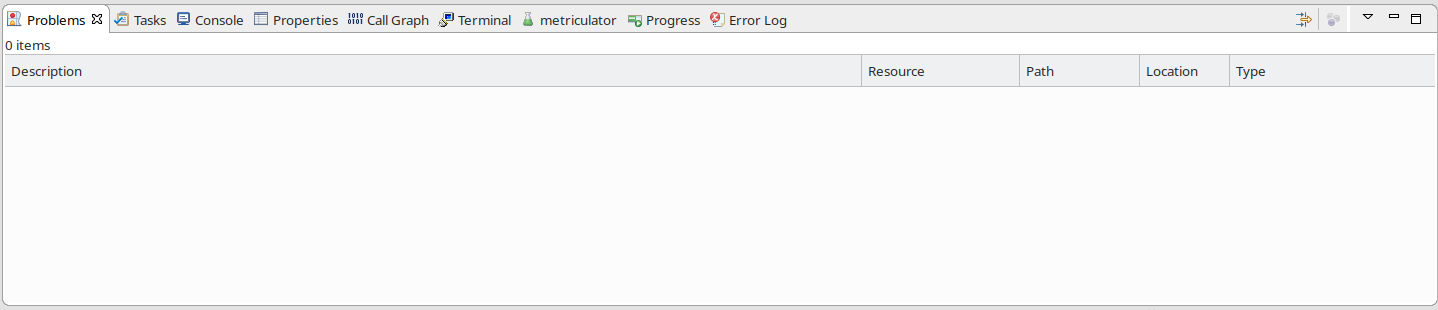
\includegraphics[scale=0.32]{img/captura96.png}
 			\caption{Captura de pantalla de los resultados arrojados tras la ejecución de cppcheck.}
 			\label{captura96}
 		\end{figure}
 	
 		\paragraph{}Respecto a los resultados arrojados por metriculator, podemos observar que aparecen tres módulos que presentan un V(G)$>$10 en la métrica de McCabe:
 		
 		\begin{itemize}
 			\item void Aplication::aplicacion\_admin()
 			\item void Aplication::aplicacion\_usuario()
 			\item void Fecha::comprobarFecha(unsigned aDia, unsigned aMes, unsigned aAnio, unsigned aHora, unsigned aMin) const
 		\end{itemize}
 		
 		
 	\subsection{Corrección del módulo $"void$ $Aplication::aplicacion\_admin()"$}
 	
 		\subsubsection{Estado del módulo antes de la corrección}
 		
 		\paragraph{}Este módulo se encuentra implementado en la línea 38 del archivo Aplication.cpp del proyecto. Su complejidad ciclomática es de V(G)=34 en la métrica de McCabe. En las siguientes capturas de pantalla se puede observar el estado de dicho módulo antes de realizar las correcciones oportunas.
 		
 		\begin{figure}[H]
 			\centering
 			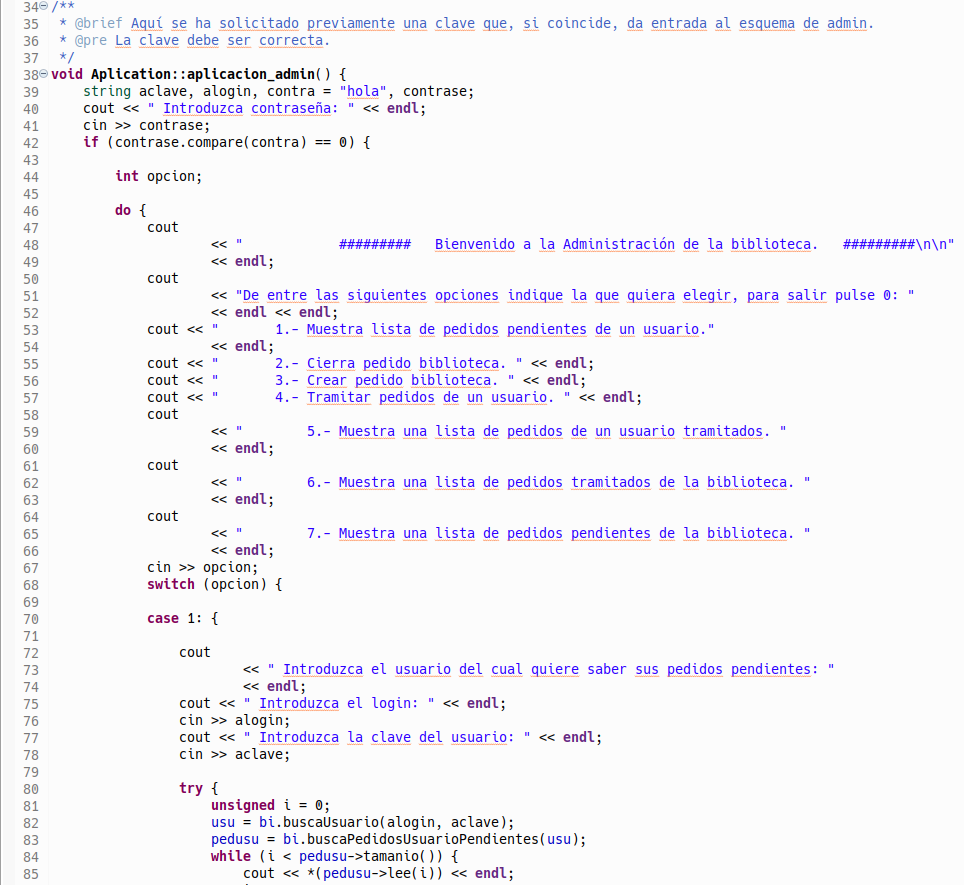
\includegraphics[scale=0.45]{img/captura97.png}
 			\caption{Detalle del módulo a corregir.}
 			\label{captura97}
 		\end{figure}
 	
 		\begin{figure}[H]
 			\centering
 			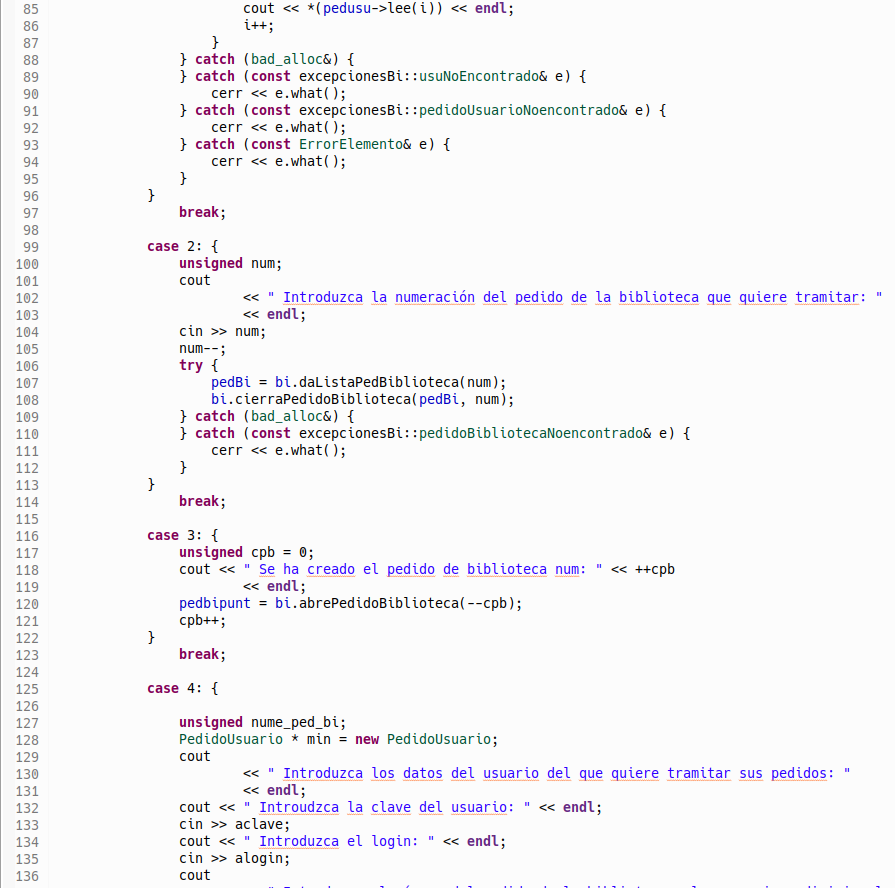
\includegraphics[scale=0.45]{img/captura98.png}
 			\caption{Detalle del módulo a corregir.}
 			\label{captura98}
 		\end{figure}
 	
 		\begin{figure}[H]
 			\centering
 			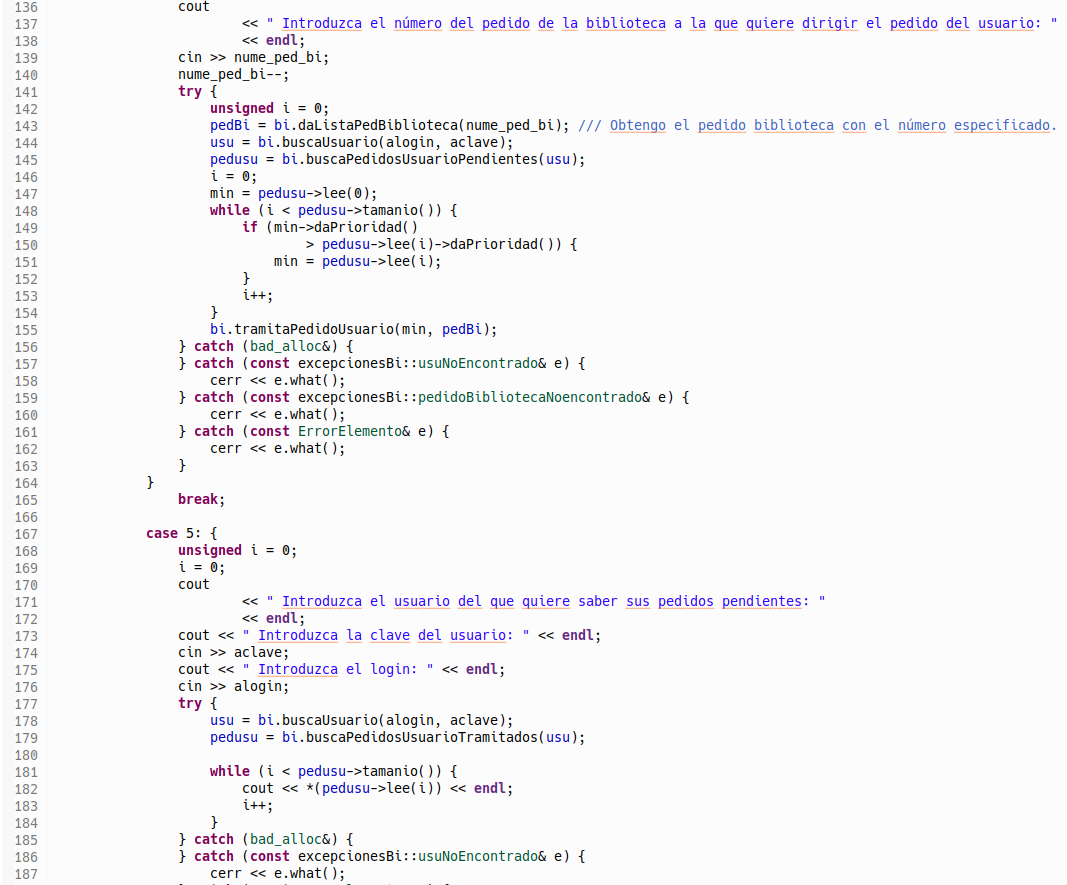
\includegraphics[scale=0.45]{img/captura99.png}
 			\caption{Detalle del módulo a corregir.}
 			\label{captura99}
 		\end{figure}
 		
 		\begin{figure}[H]
 			\centering
 			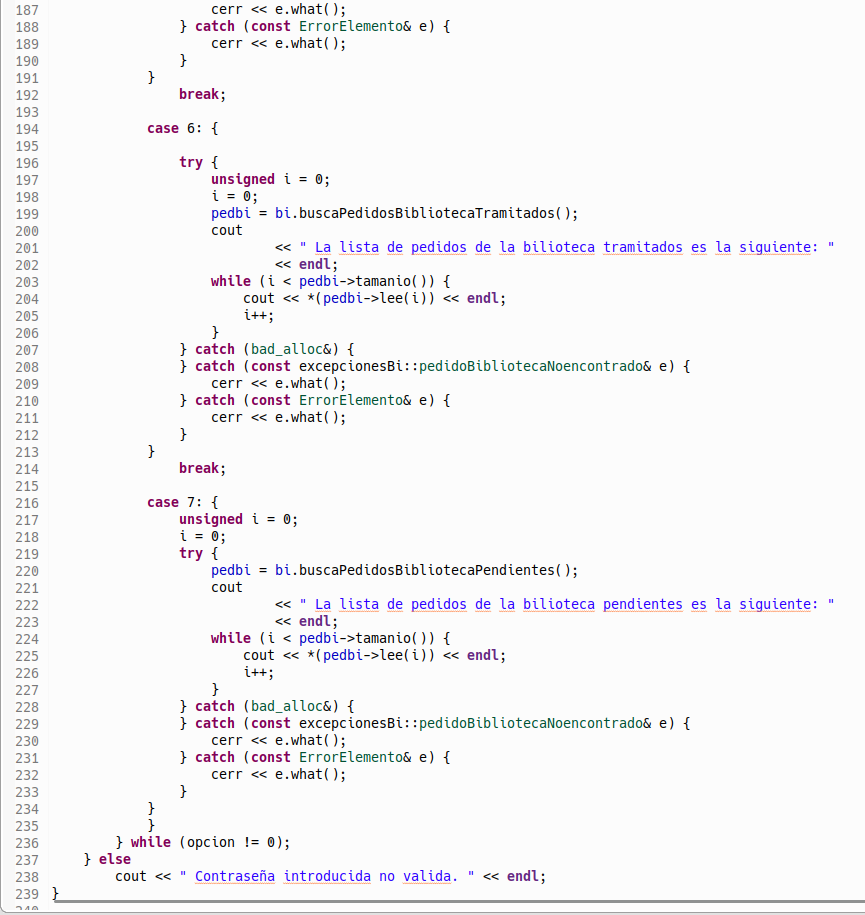
\includegraphics[scale=0.5]{img/captura100.png}
 			\caption{Detalle del módulo a corregir.}
 			\label{captura100}
 		\end{figure}
 	
 		\subsubsection{Estado del módulo después de la corrección}
 		
 			\paragraph{}Como se puede observar en las capturas de pantalla del módulo en el apartado anterior se trata de un módulo con un altísimo número de líneas de código. Una primera estrategia que seguiremos será la de modularizar parte de este código.
 			
 			\paragraph{}En concreto, modularizaremos el código que se encuentra en cada uno de los \textit{case} para reducir la complejidad y la legibilidad del código. Una vez hecho esto, se crearán las siguientes funciones:
 			
 			\begin{itemize}
 				\item void Aplication::mostrarMenu()
 				\item void Aplication::mostrarListaPedidosPendientes(string alogin, string aclave)
 				\item void Aplication::mostrarTramitarPedido()
 				\item void Aplication::mostrarTramitarPedidosUsuario(string alogin, string aclave)
 				\item void Aplication::mostrarConsultarPedidosUsuario(string alogin, string aclave)
 				\item void Aplication::mostrarListaPedidosTramitados()
 				\item void Aplication::mostrarListaPedidosPendientesBiblioteca()
 			\end{itemize}
 		
 			\paragraph{}A continuación, presentamos capturas de pantalla de todos los módulos enumerados anteriormente.
 			
 			\begin{figure}[H]
 				\centering
 				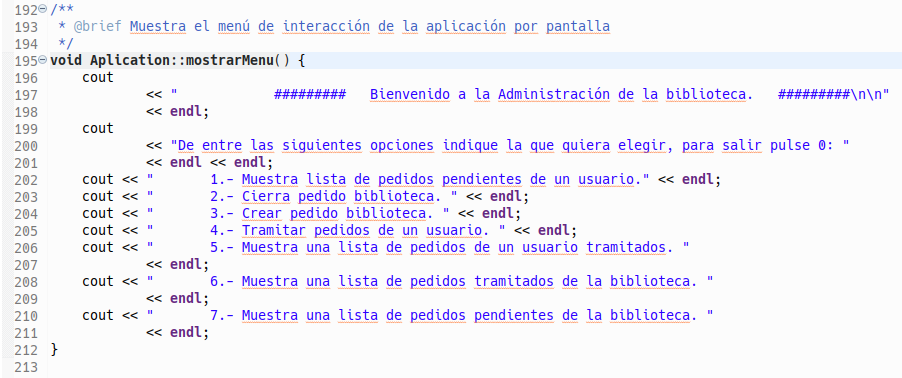
\includegraphics[scale=0.5]{img/captura101.png}
 				\caption{Detalle del módulo mostrarMenu.}
 				\label{captura101}
 			\end{figure}
 			
 			\begin{figure}[H]
 				\centering
 				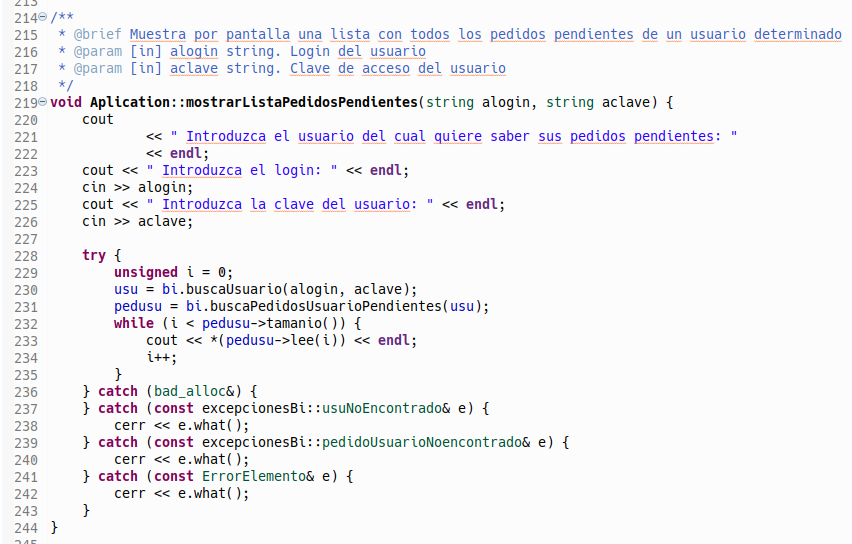
\includegraphics[scale=0.5]{img/captura102.png}
 				\caption{Detalle del módulo mostrarListaPedidosPendientes.}
 				\label{captura102}
 			\end{figure}
 		
 			\begin{figure}[H]
 				\centering
 				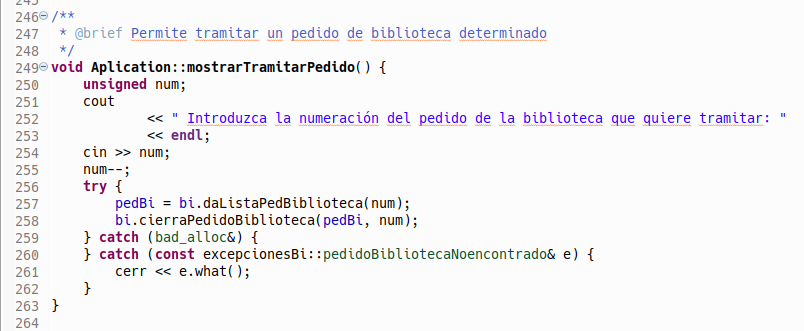
\includegraphics[scale=0.5]{img/captura103.png}
 				\caption{Detalle del módulo mostrarTramitarPedido.}
 				\label{captura103}
 			\end{figure}
 		
 			\begin{figure}[H]
 				\centering
 				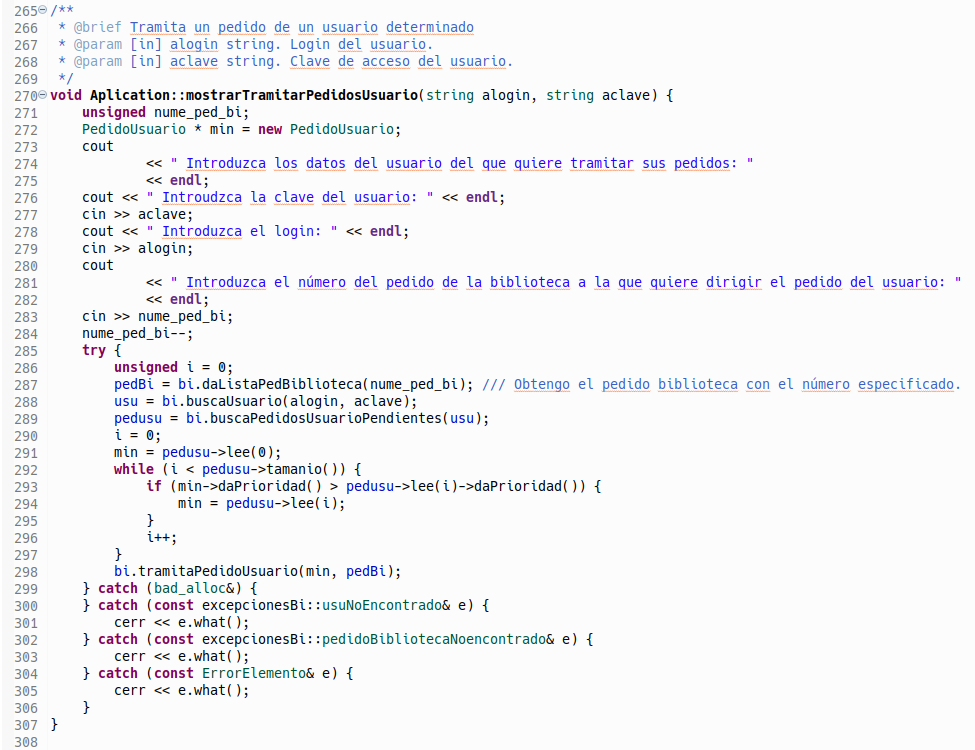
\includegraphics[scale=0.5]{img/captura104.png}
 				\caption{Detalle del módulo mostrarTramitarPedidosUsuario.}
 				\label{captura104}
 			\end{figure}
			
			\begin{figure}[H]
				\centering
				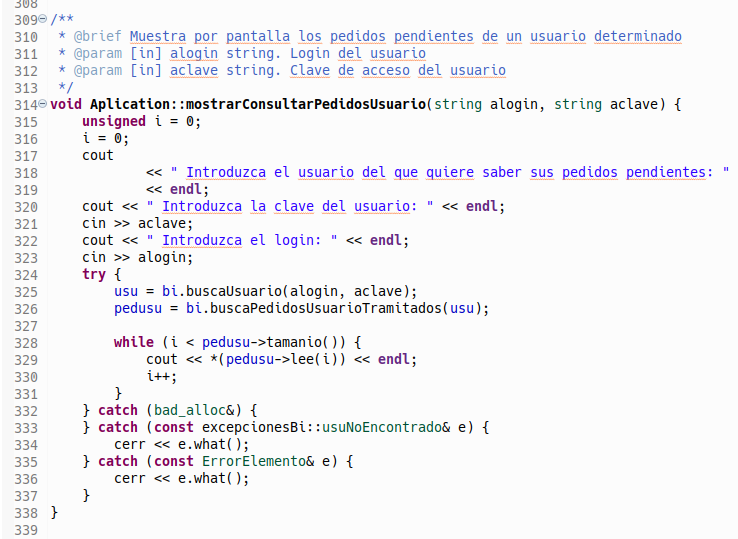
\includegraphics[scale=0.5]{img/captura105.png}
				\caption{Detalle del módulo mostrarConsultarPedidosUsuario.}
				\label{captura105}
			\end{figure}
		
			\begin{figure}[H]
				\centering
				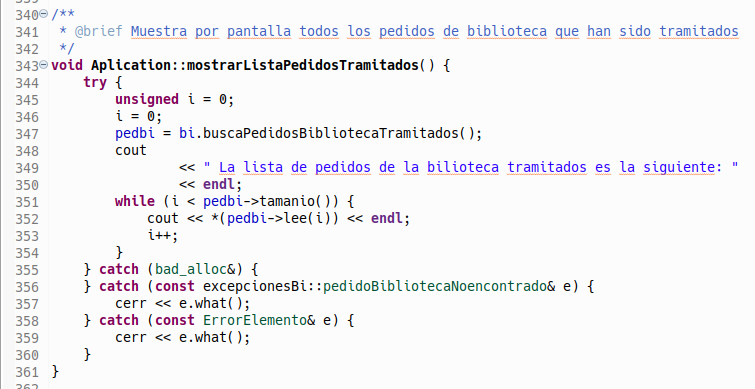
\includegraphics[scale=0.5]{img/captura106.png}
				\caption{Detalle del módulo mostrarListaPedidosTramitados.}
				\label{captura106}
			\end{figure}
		
			\begin{figure}[H]
				\centering
				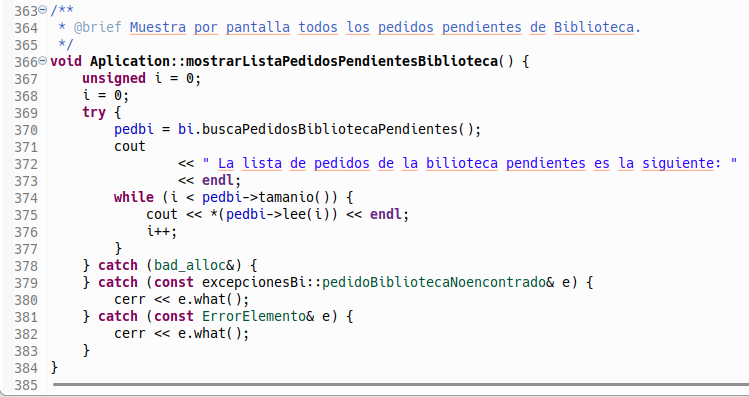
\includegraphics[scale=0.5]{img/captura107.png}
				\caption{Detalle del módulo mostrarListaPedidosPendientesBiblioteca.}
				\label{captura107}
			\end{figure}
		
			\paragraph{}Una vez creados todos los anteriores módulos el estado del módulo a corregir es el que se muestra en la siguiente captura de pantalla.
			
			\begin{figure}[H]
				\centering
				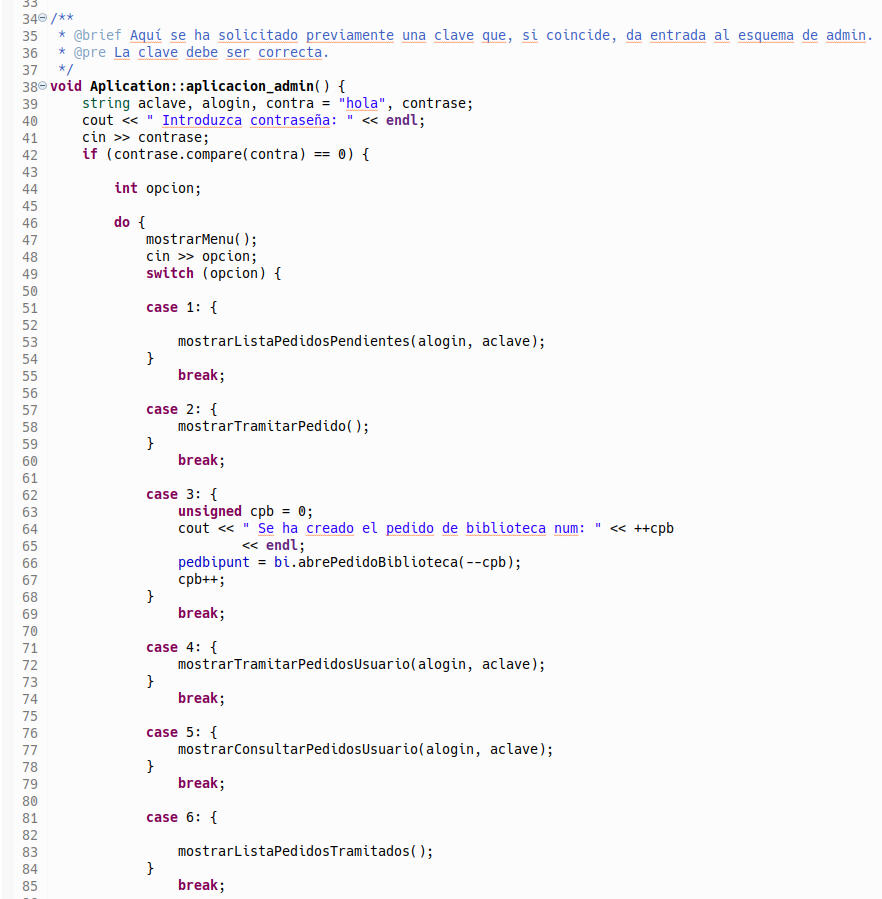
\includegraphics[scale=0.5]{img/captura108.png}
				\caption{Detalle del módulo corregido.}
				\label{captura108}
			\end{figure}
			
			\begin{figure}[H]
				\centering
				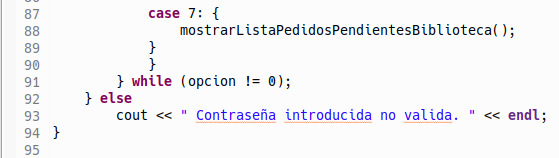
\includegraphics[scale=0.7]{img/captura109.png}
				\caption{Detalle del módulo corregido.}
				\label{captura109}
			\end{figure}
		
			\paragraph{}A continuación, realizamos un nuevo análisis de metriculator para comprobar en que grado hemos disminuido V(G). Obtenemos los siguientes resultados.
			
			\begin{figure}[H]
				\centering
				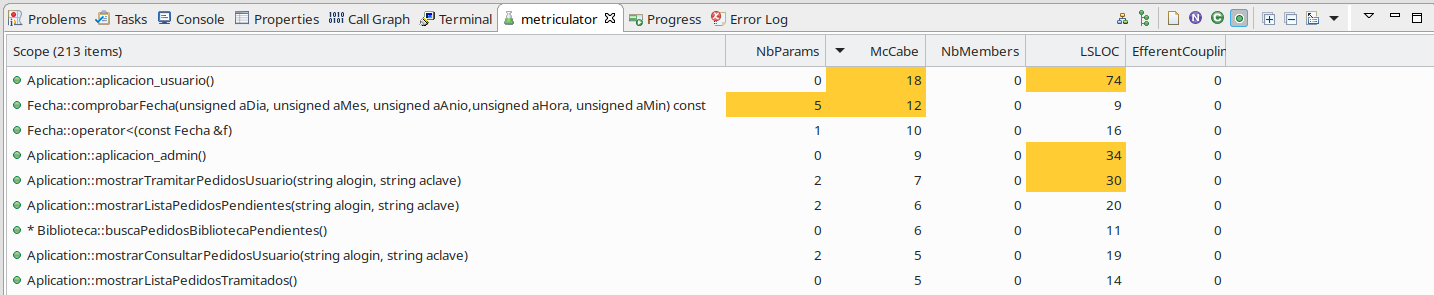
\includegraphics[scale=0.32]{img/captura110.png}
				\caption{Resultados de metriculator tras las correcciones realizadas.}
				\label{captura110}
			\end{figure}
		
			\paragraph{}Podemos comprobar que hemos conseguido obtener un V(G)=9 en la métrica de McCabe, por lo que hemos conseguido cumplir con el objetivo de la corrección.
			
			\paragraph{}Para terminar, ejecutamos un nuevo test de cppcheck para comprobar que no arrastremos ningún error o warning en las funciones nuevas. Obtenemos los siguientes resultados.
			
			\begin{figure}[H]
				\centering
				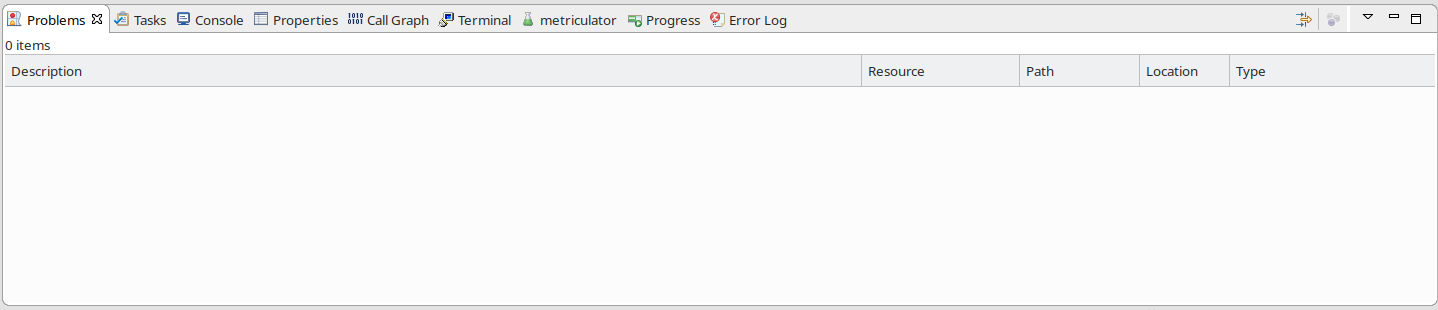
\includegraphics[scale=0.32]{img/captura96.png}
				\caption{Resultados de cppcheck tras las correcciones realizadas.}
				\label{captura111}
			\end{figure}
		
			\paragraph{}Podemos observar que no obtenemos ningún error, warning o aviso; por lo tanto, damos por concluida la corrección del módulo.
			
	\subsection{Corrección del módulo $"void$ $Aplication::aplicacion\_usuario()"$}
	
	\subsubsection{Estado del módulo antes de la corrección}
	
		\paragraph{}Este módulo se encuentra implementado en la línea 100 del archivo Aplication.cpp del proyecto. Su complejidad ciclomática es de V(G) = 18 en la métrica de McCabe. En las siguientes capturas de pantalla se puede observar el estado de dicho módulo antes de realizar las correcciones oportunas.
		
		\begin{figure}[H]
			\centering
			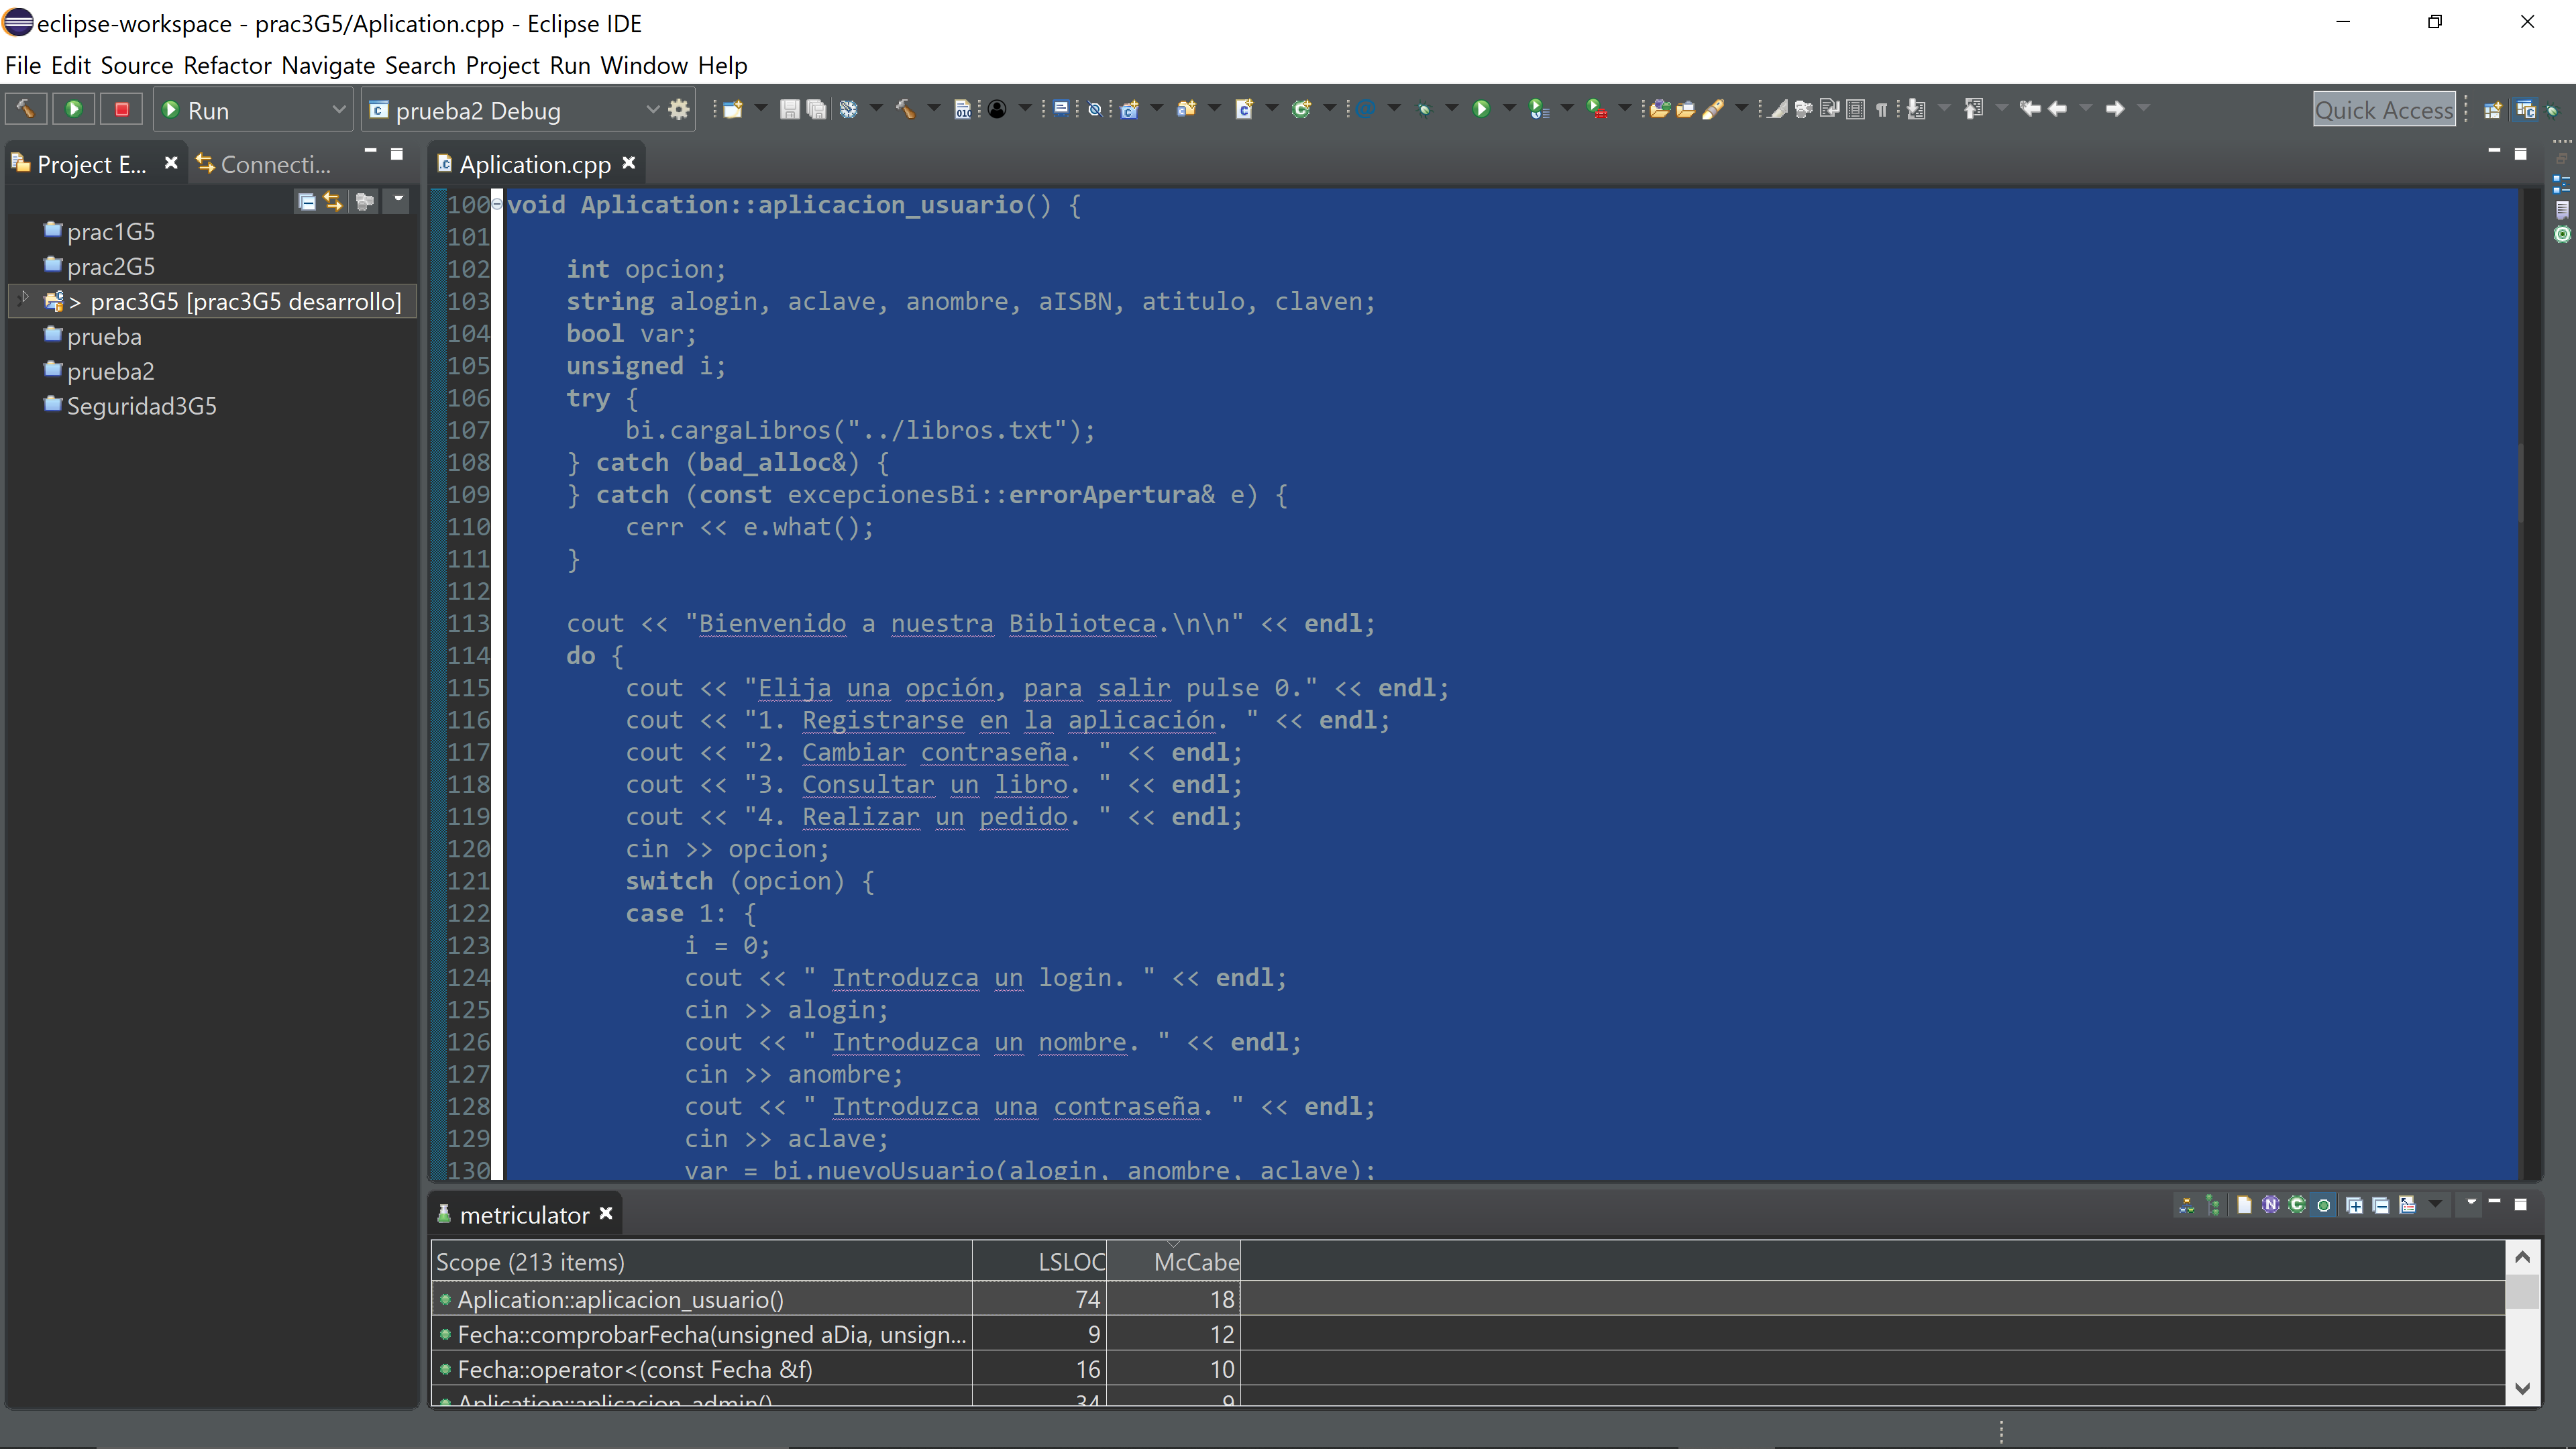
\includegraphics[scale=0.1]{img/estebanFinal1.png}
			\caption{Detalles del módulo a corregir.}
			\label{estebanFinal1}
		\end{figure}
	
		\begin{figure}[H]
			\centering
			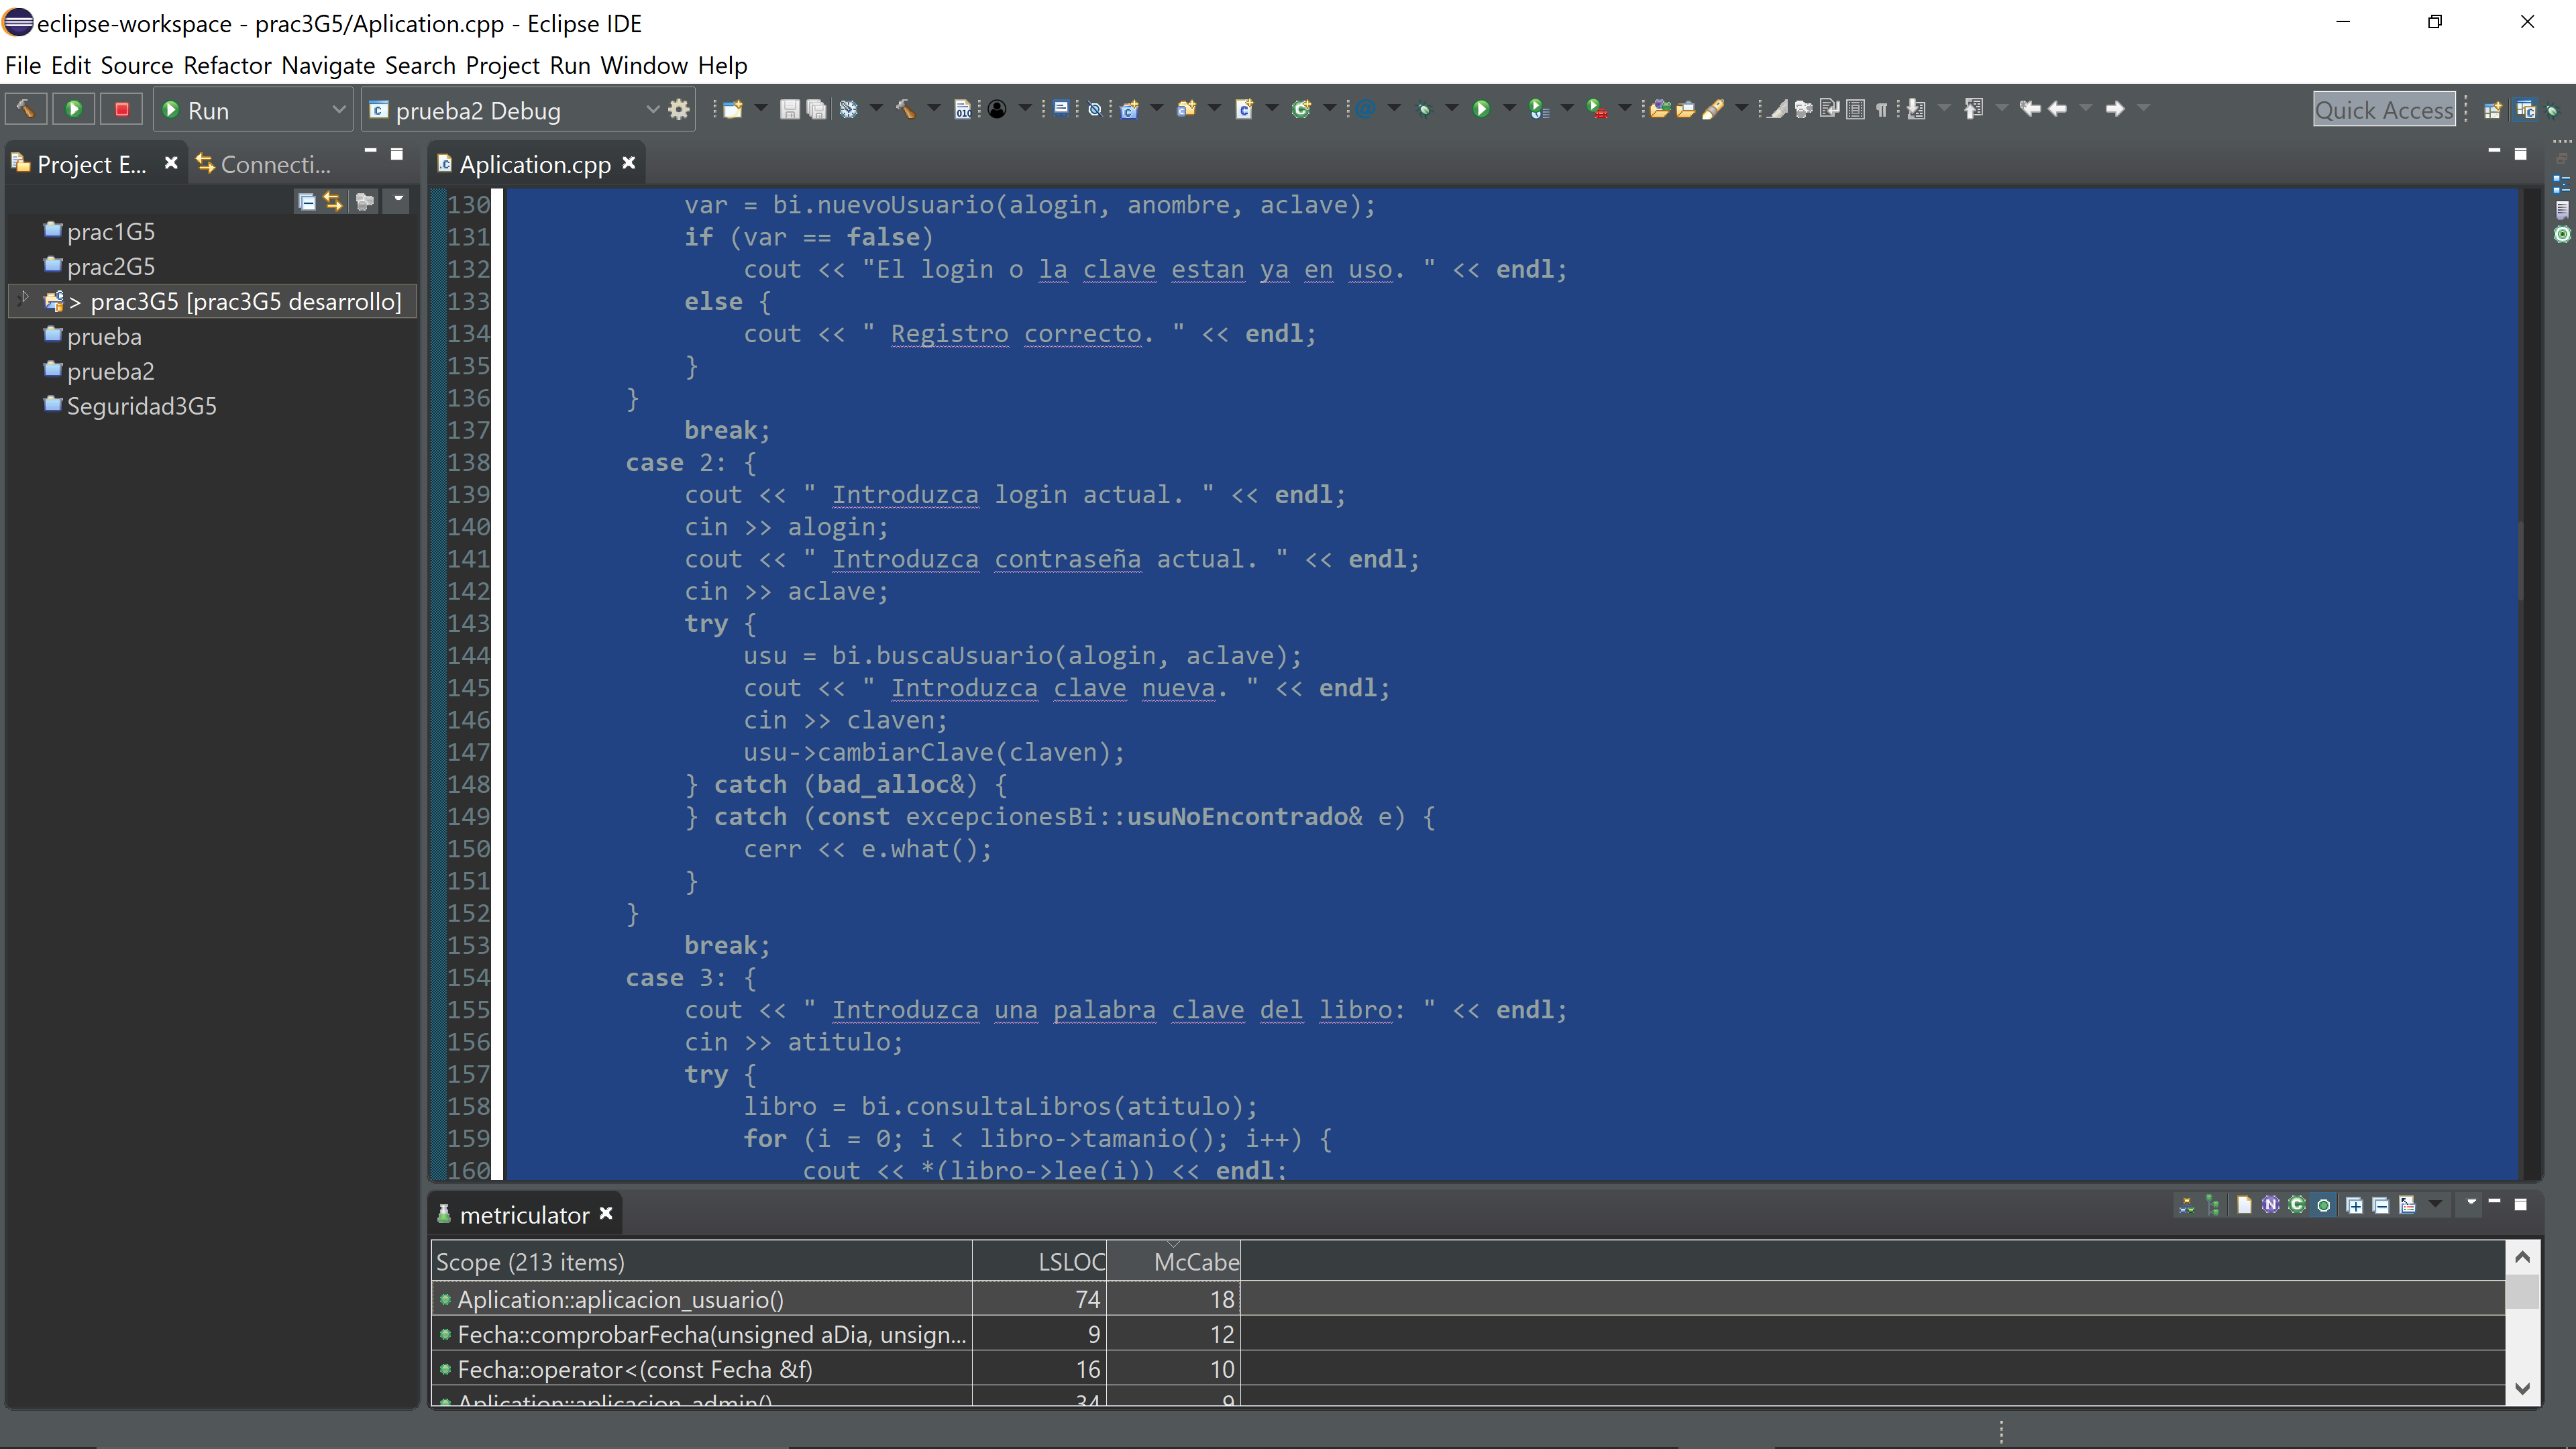
\includegraphics[scale=0.1]{img/estebanFinal2.png}
			\caption{Detalles del módulo a corregir.}
			\label{estebanFinal2}
		\end{figure}
	
		\begin{figure}[H]
			\centering
			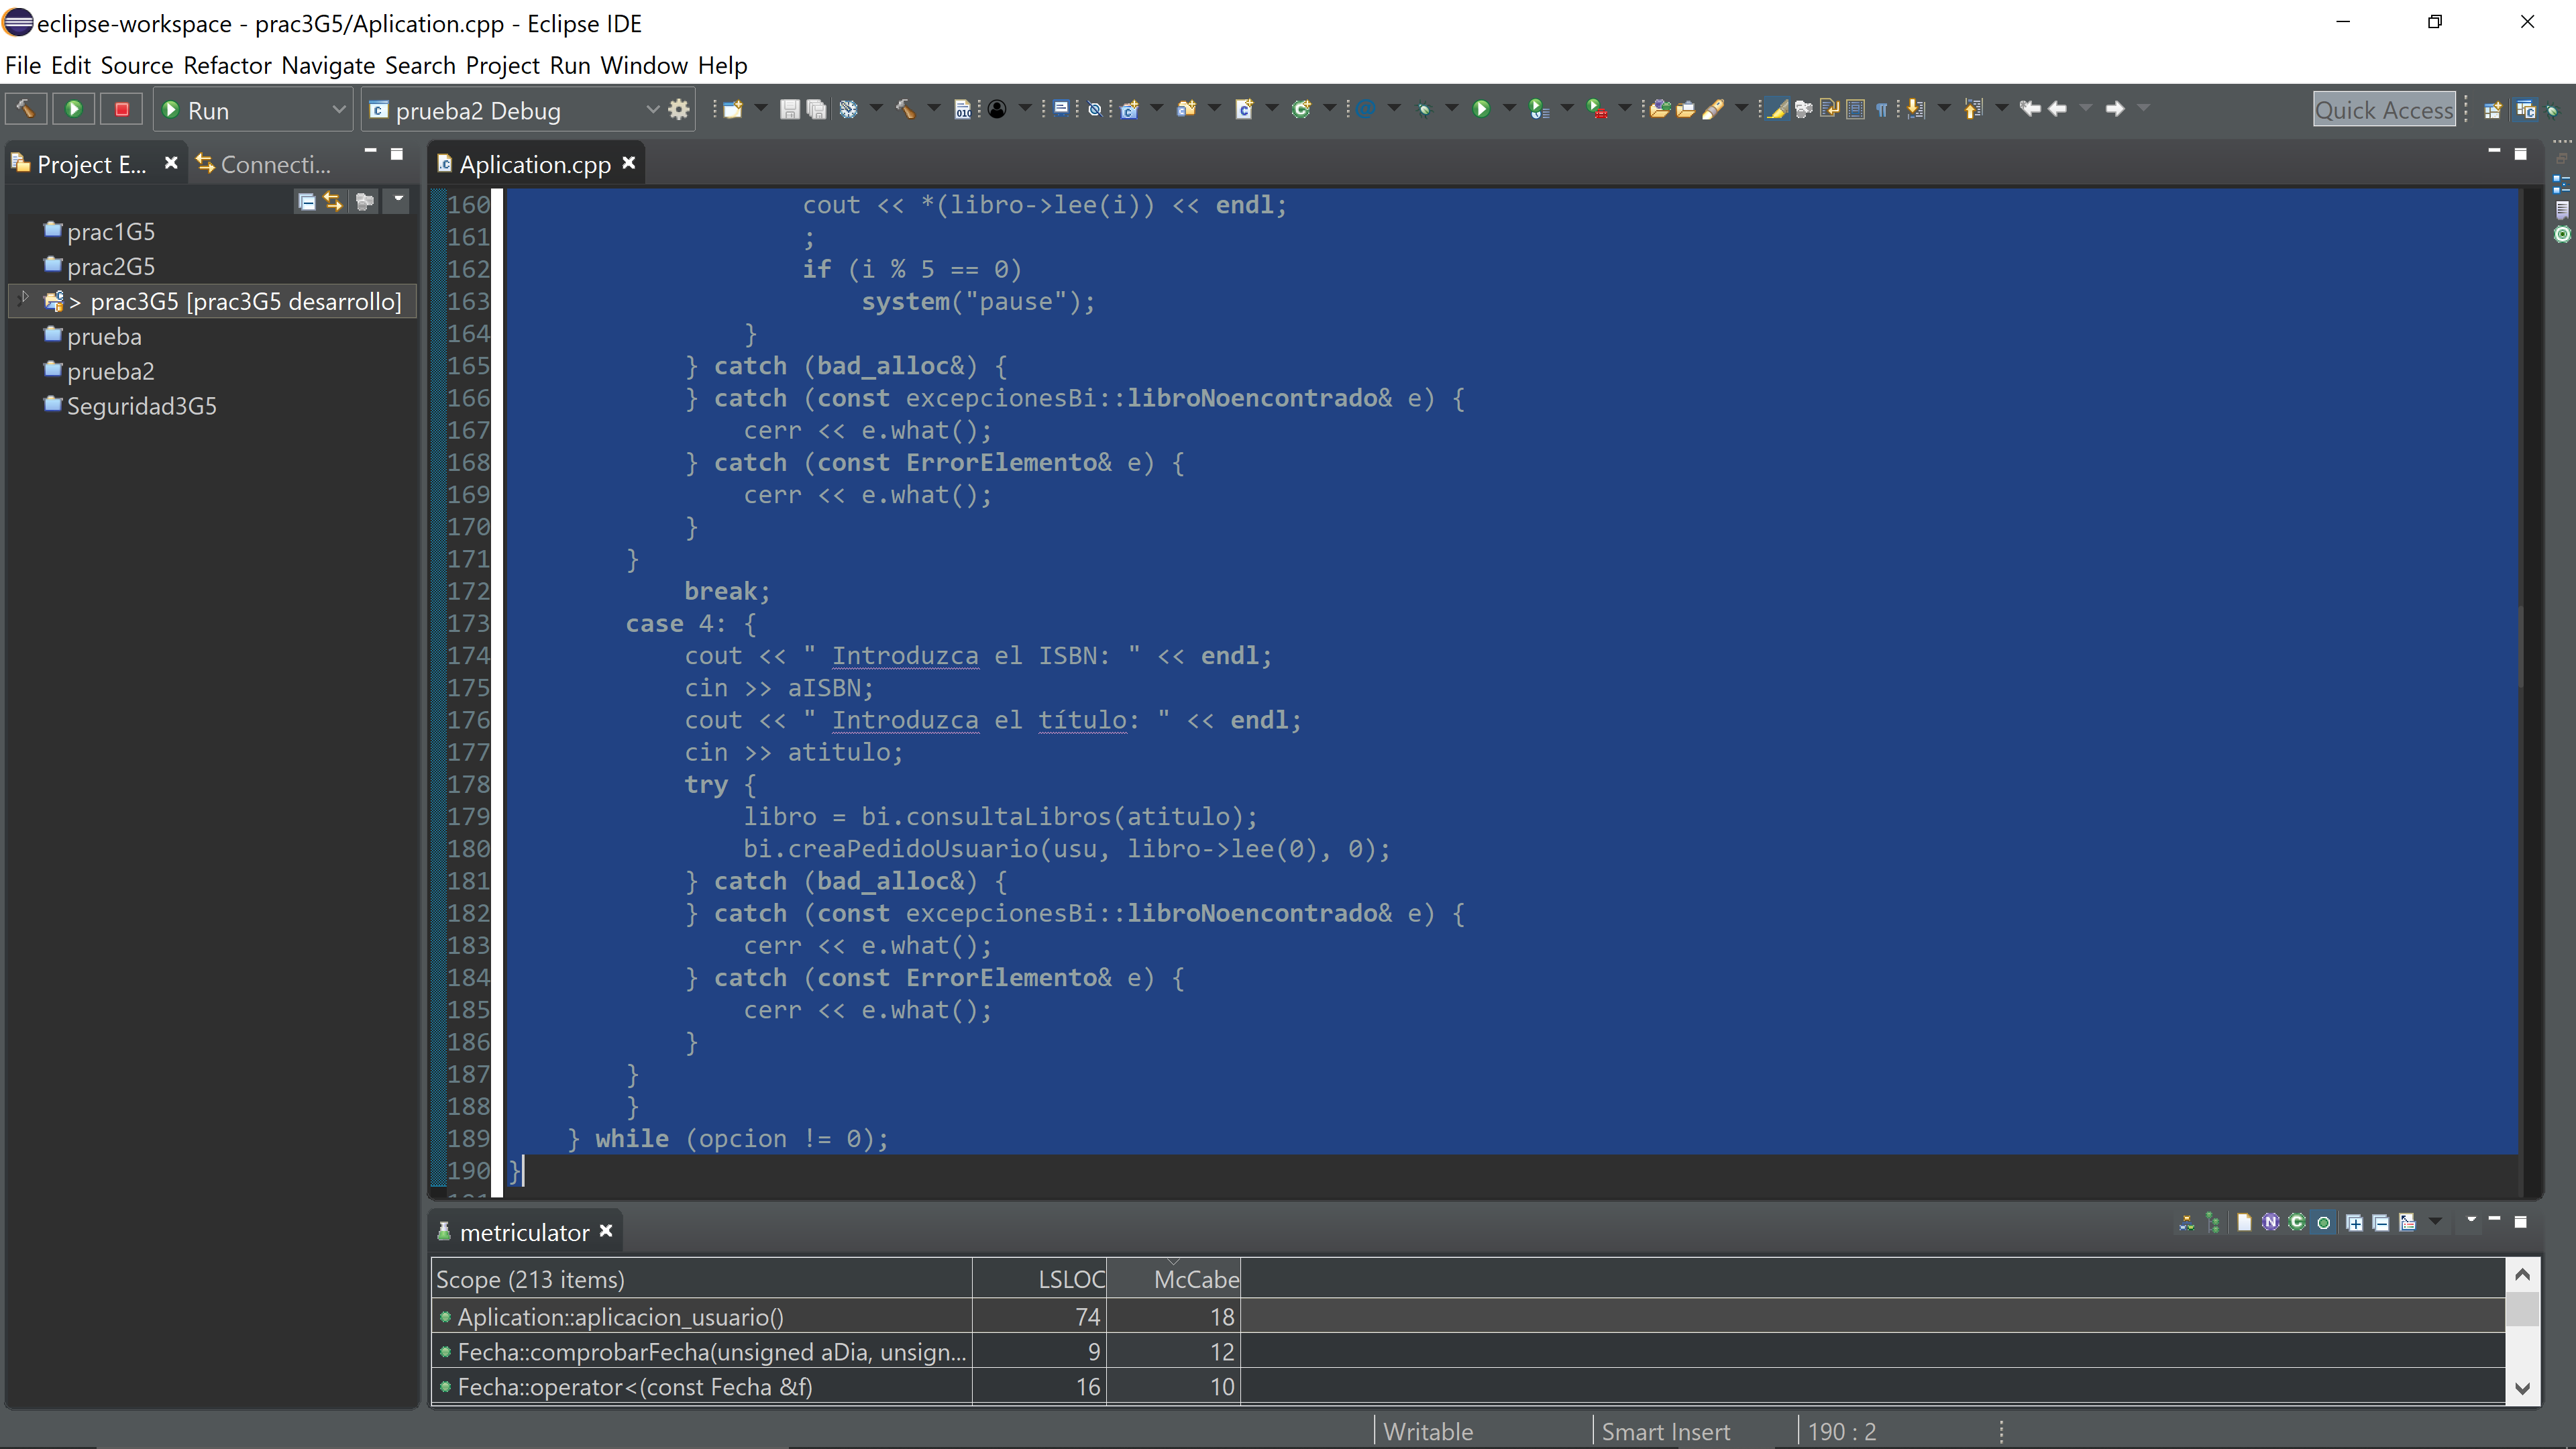
\includegraphics[scale=0.1]{img/estebanFinal3.png}
			\caption{Detalles del módulo a corregir.}
			\label{estebanFinal3}
		\end{figure}
		
		\paragraph{}Como hemos procedido anteriormente, modularizaremos el código que se encuentra en cada uno de los case para reducir la complejidad y la legibilidad del código. Una vez hecho esto, se crearán las siguientes funciones:
		
		\begin{itemize}
			\item void Aplication::mostrarMenuUsuario();
			
			\begin{figure}[H]
				\centering
				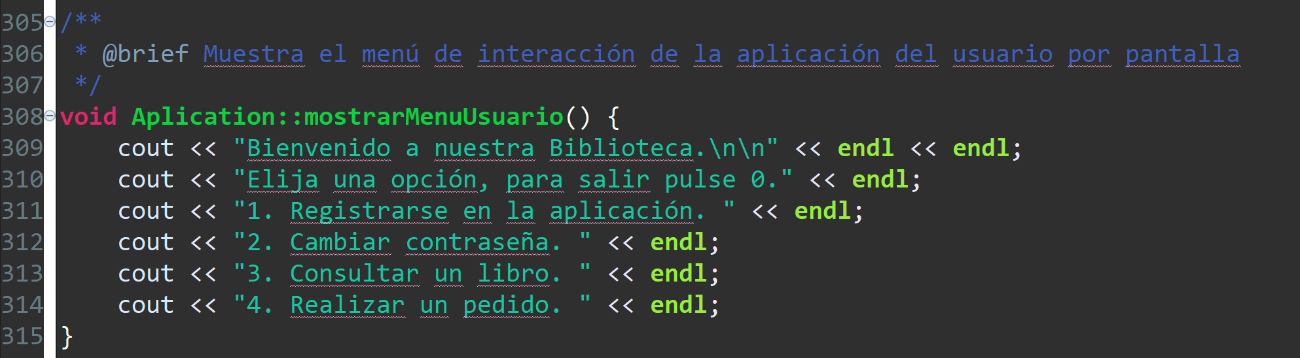
\includegraphics[scale=0.9]{img/estebanFinal4.png}
				\caption{Detalles del módulo mostrarMenuUsuario.}
				\label{estebanFinal4}
			\end{figure}
		
			\item void Aplication::registro(string alogin, string aclave, string aclave);
			
			\begin{figure}[H]
				\centering
				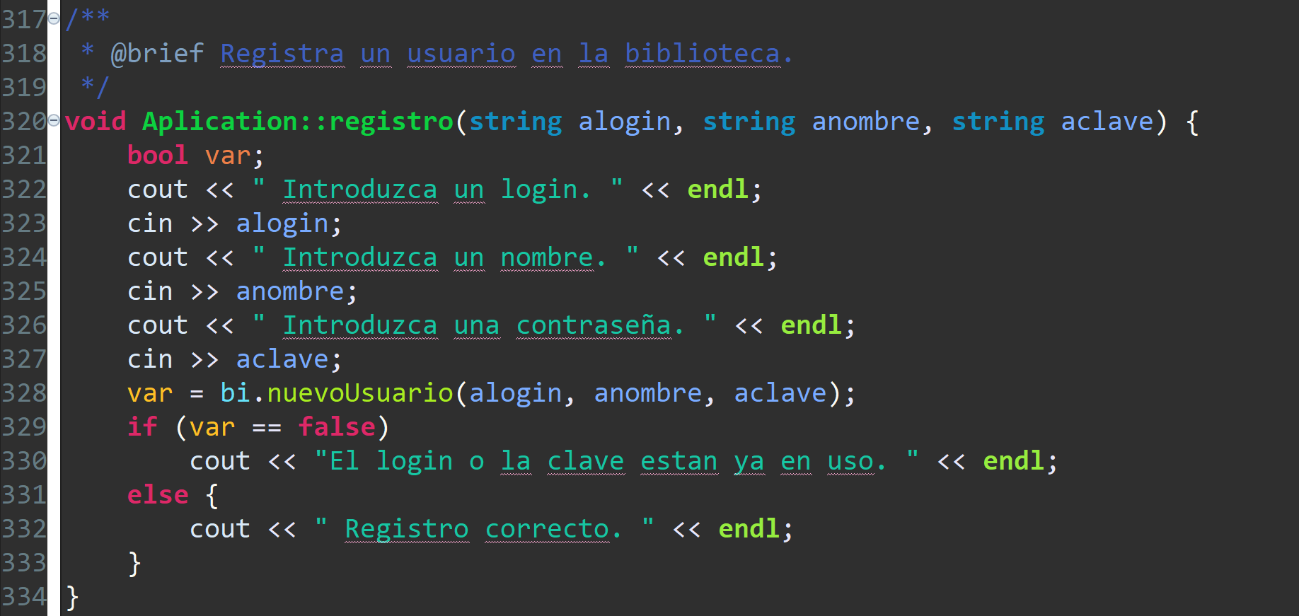
\includegraphics[scale=0.9]{img/estebanFinal5.png}
				\caption{Detalles del módulo registro.}
				\label{estebanFinal5}
			\end{figure}
		
			\item void Aplication::cambiaClave(string alogin, string aclave, string claven);
			
			\begin{figure}[H]
				\centering
				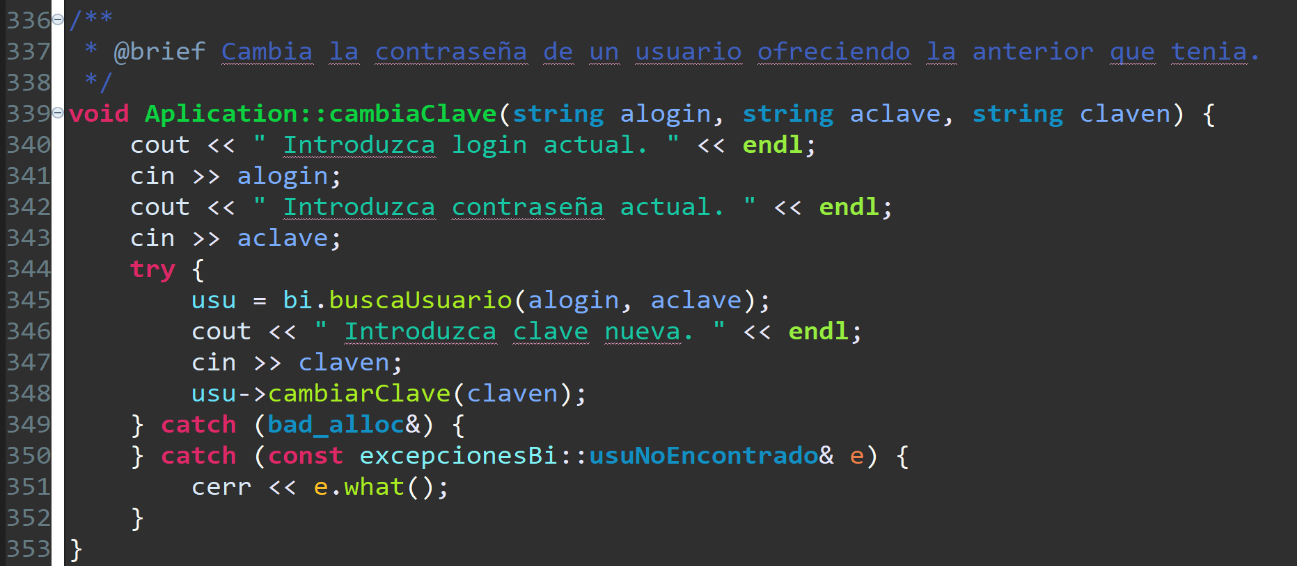
\includegraphics[scale=0.9]{img/estebanFinal6.png}
				\caption{Detalles del módulo cambiaClave.}
				\label{estebanFinal6}
			\end{figure}
		
			\item void Aplication::consultaLibro(string atitulo);
			
			\begin{figure}[H]
				\centering
				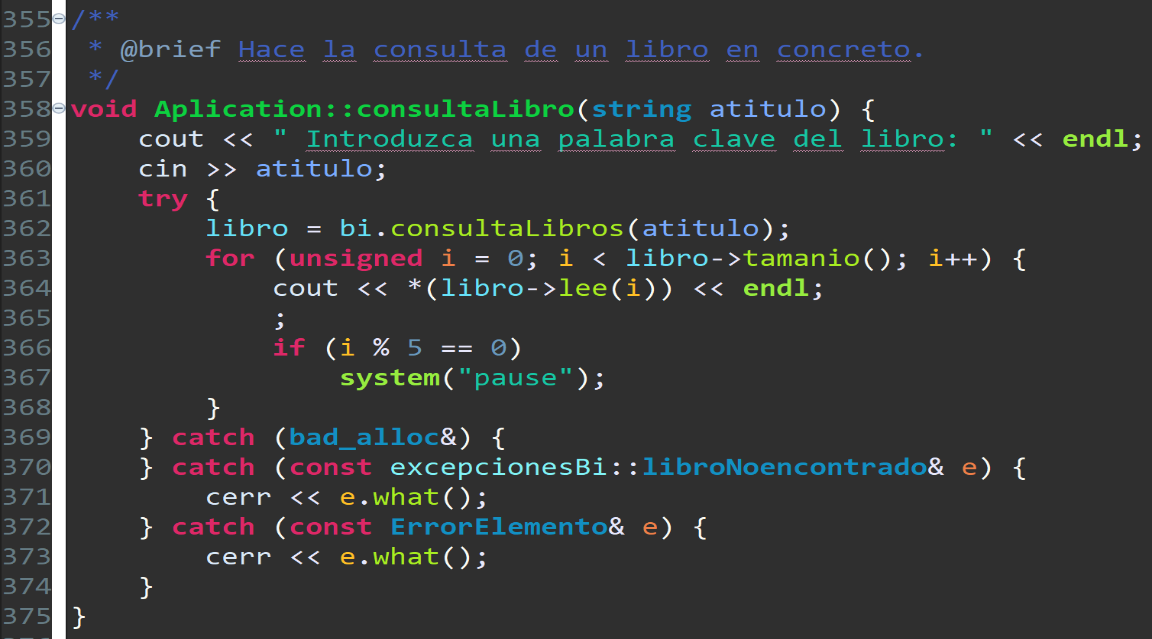
\includegraphics[scale=0.9]{img/estebanFinal7.png}
				\caption{Detalles del módulo consultaLibro.}
				\label{estebanFinal7}
			\end{figure}
		
			\item void Aplication::hazPedido(string aISBN, string atitulo);
		\end{itemize}
	
			\begin{figure}[H]
				\centering
				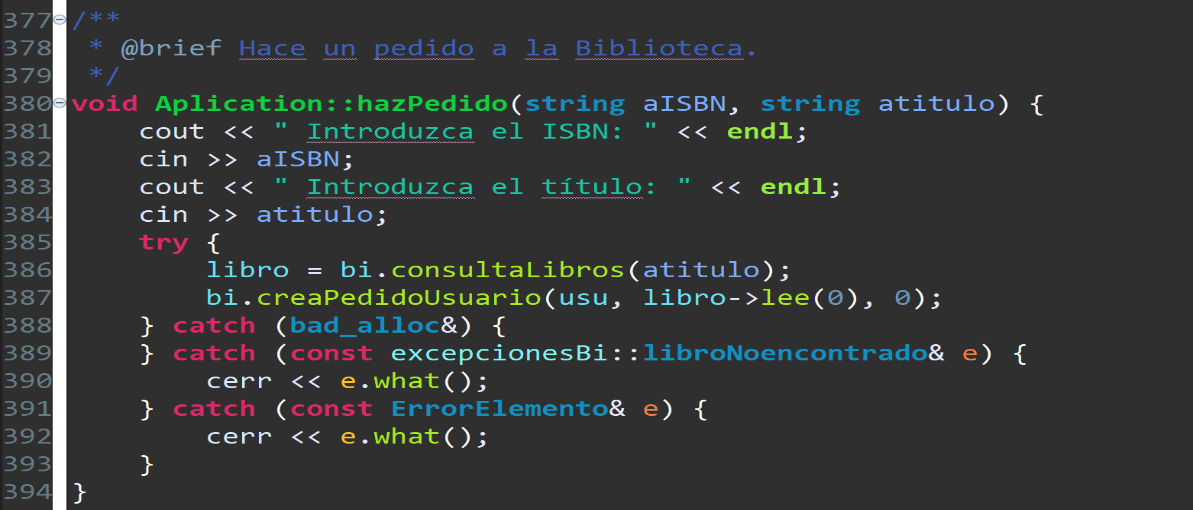
\includegraphics[scale=0.9]{img/estebanFinal8.png}
				\caption{Detalles del módulo hazPedido.}
				\label{estebanFinal8}
			\end{figure}
	
	\subsubsection{Estado del módulo después de la corrección}
	
		\paragraph{}Una vez creados todos los anteriores módulos el estado del módulo a corregir es el que se muestra en la siguiente captura de pantalla.
		
		\begin{figure}[H]
			\centering
			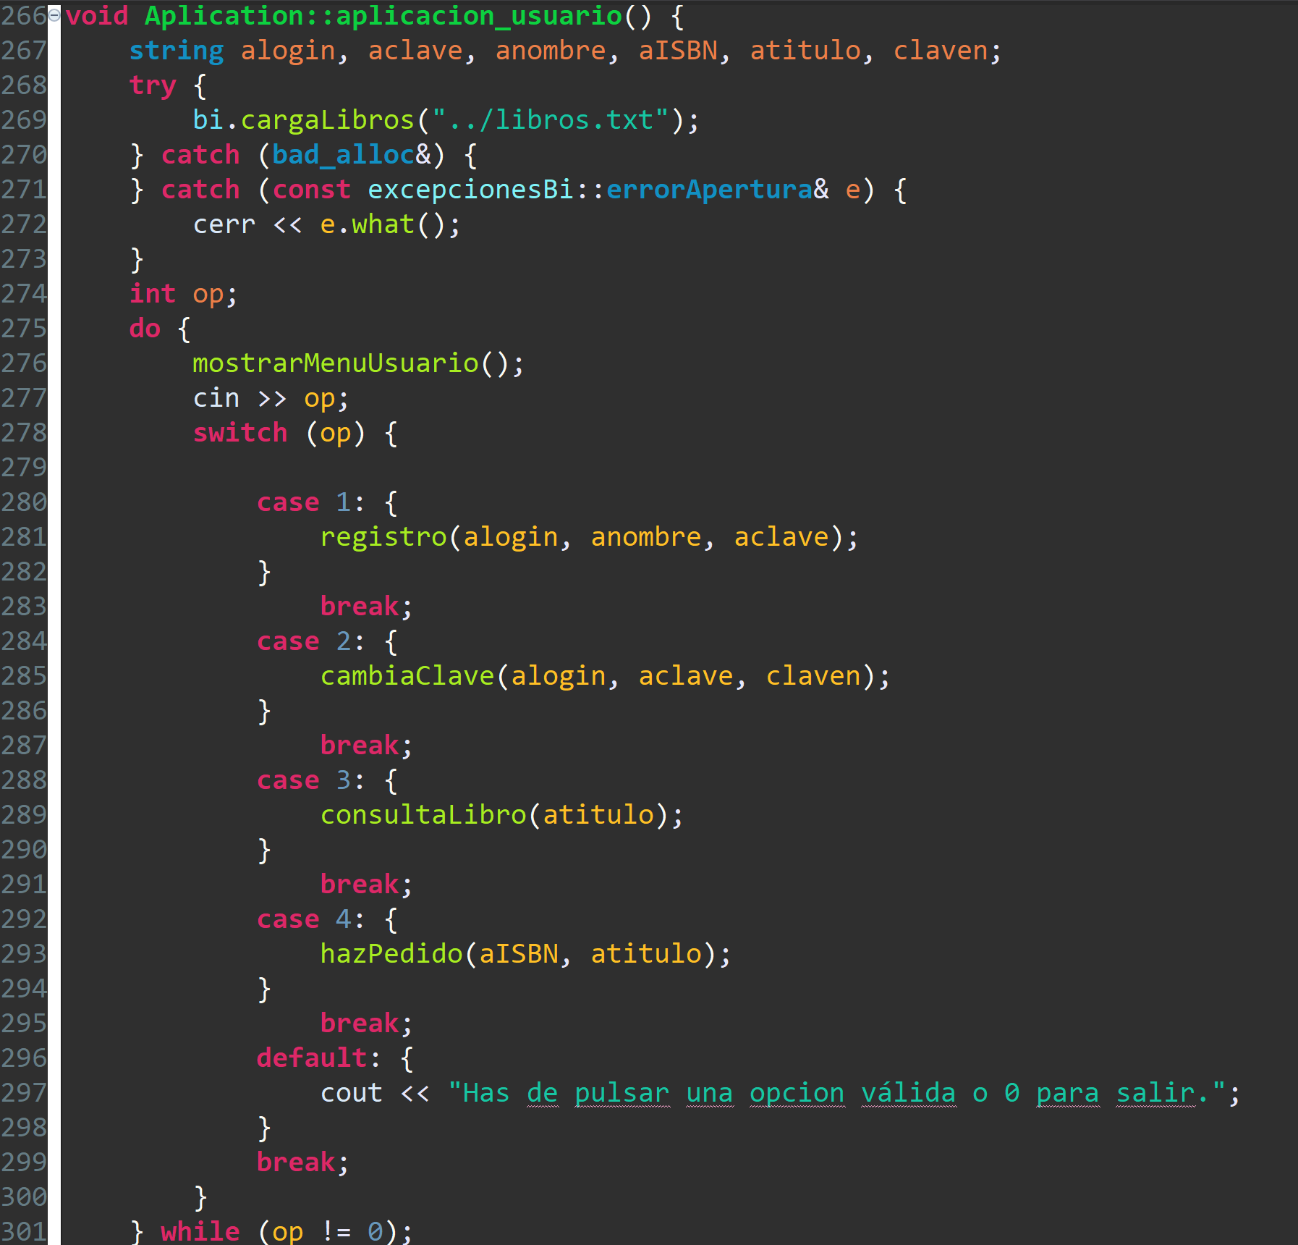
\includegraphics[scale=0.9]{img/estebanFinal9.png}
			\caption{Detalles del módulo corregido.}
			\label{estebanFinal9}
		\end{figure}
		
		\paragraph{}A continuación, realizamos un nuevo análisis de metriculator para comprobar en qué grado hemos disminuido V(G). Obtenemos los siguientes resultados.
		
		\begin{figure}[H]
			\centering
			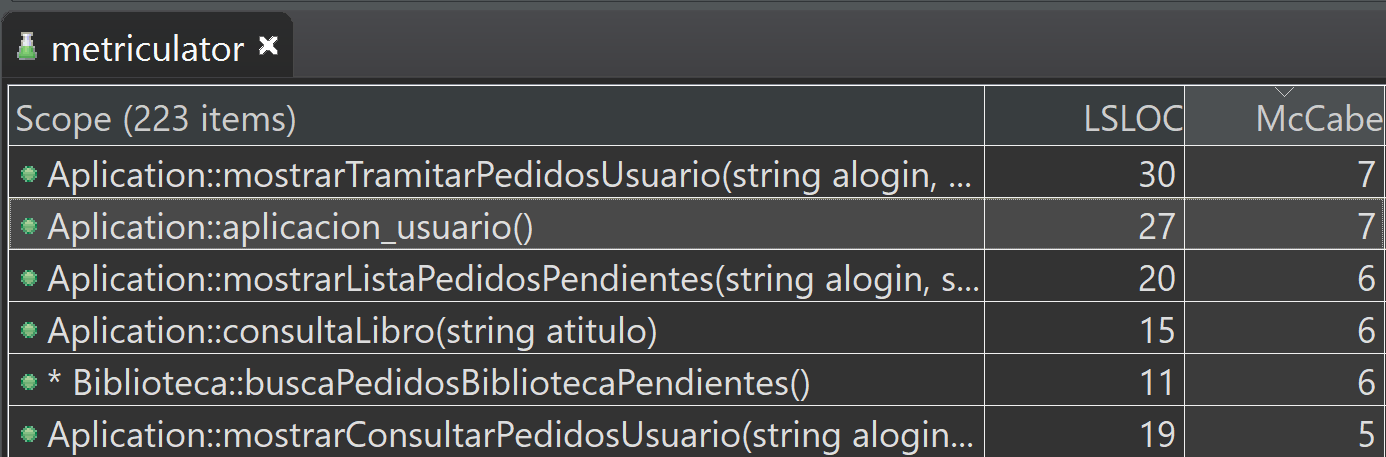
\includegraphics[scale=0.9]{img/estebanFinal10.png}
			\caption{Resultados de metriculator tras las correcciones realizadas.}
			\label{estebanFinal10}
		\end{figure}
		
		\paragraph{}Con lo cual hemos reducido V(g) de 18 a 7 en void Aplication :: aplicacion usuario();
	
	\subsection{Corrección del módulo $"void$ $Fecha::comprobarFecha(unsigned$ $aDia,$ $unsigned$ $aMes,$ $unsigned$ $aAnio,$ $unsigned$ $aHora,$ $unsigned$ $aMin)$ $const"$}
	
	\subsubsection{Estado del módulo antes de la corrección}
	
	\paragraph{}Este módulo se encuentra implementado en la línea 208 del archivo Fecha.cpp del proyecto. Su complejidad ciclomática es de V(G) = 12 en la métrica de McCabe. En la siguiente captura de pantalla se puede observar el estado de dicho módulo antes de realizar las correcciones oportunas.
	
	\begin{figure}[H]
		\centering
		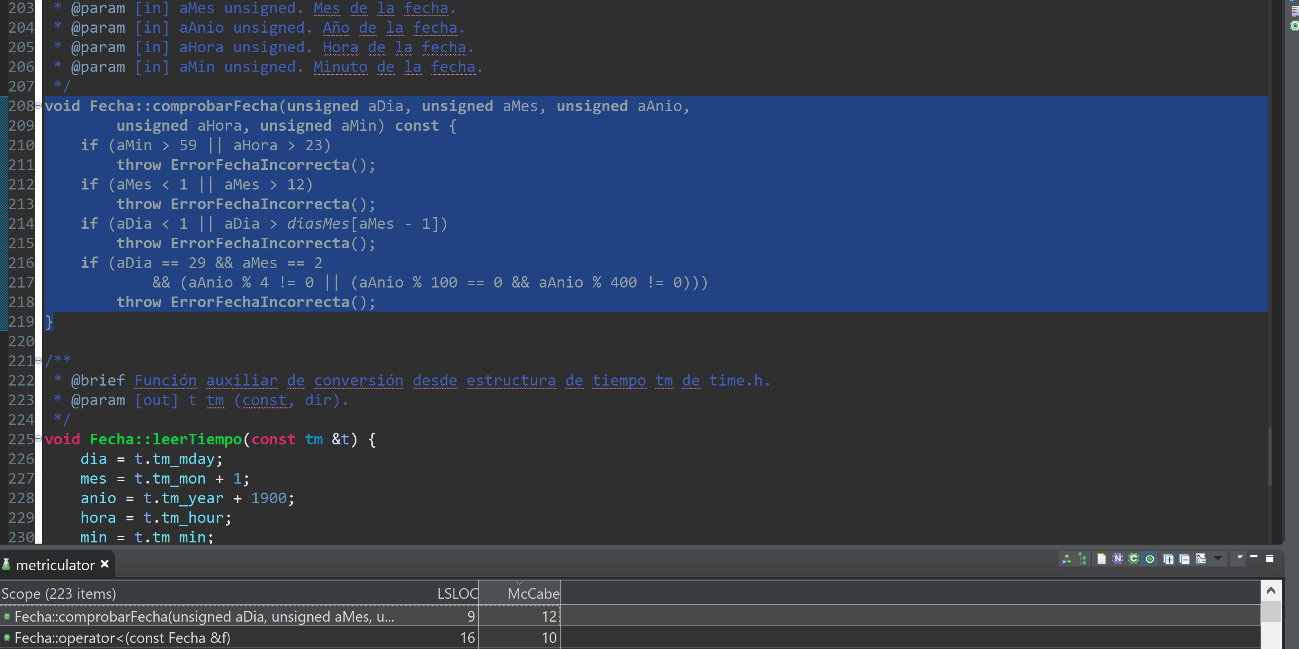
\includegraphics[scale=0.9]{img/estebanFinal11.png}
		\caption{Detalle del módulo a corregir.}
		\label{estebanFinal11}
	\end{figure}
	
	\paragraph{}La complejidad de este módulo es debido a las numerosas comprobaciones que han de hacerse. Además, la gran cantidad de operadores tales como $|$$|$, \&\&, $<$, $>$, ==, ¡= aumentan este valor.
	
	\paragraph{}Observamos que hace la comprobación de si el año es bisiesto para añadirle un día más a febrero.
	
	\paragraph{}Se ha decidido obviar tal comprobación al parecer excesiva para el carácter de la práctica y hemos logrado reducir la V(g) del módulo de 12 hasta 10 como podemos observar en las siguientes imágenes.
	
	\subsubsection{Estado del módulo después de la corrección}
	
	\begin{figure}[H]
		\centering
		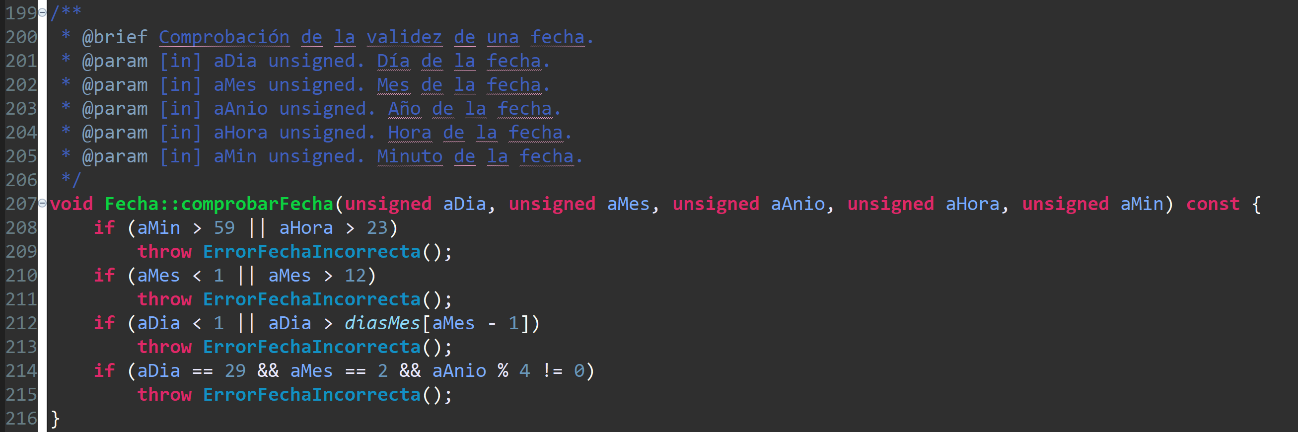
\includegraphics[scale=0.9]{img/estebanFinal12.png}
		\caption{Detalle del módulo después de aplicar las correcciones.}
		\label{estebanFinal12}
	\end{figure}

	\begin{figure}[H]
		\centering
		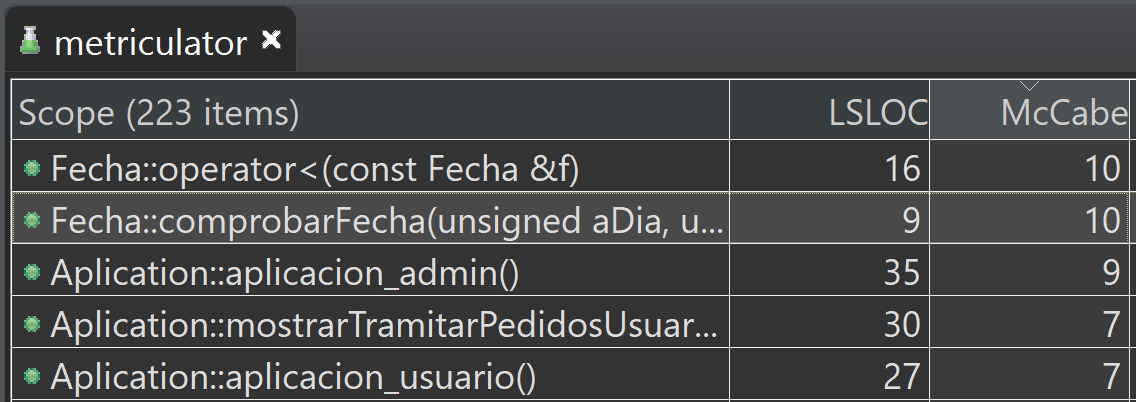
\includegraphics[scale=0.9]{img/estebanFinal13.png}
		\caption{Resultados de metriculator tras las correcciones realizadas.}
		\label{estebanFinal13}
	\end{figure}

	\subsection{Estado del proyecto después de las correcciones}
	
	\paragraph{}Tras realizar todas las correcciones que se exponen en los apartados anteriores, volvemos a ejecutar los tests de metriculator y cppcheck para comprobar el estado final del proyecto. Los resultados arrojados se exponen a continuación:
	
	\begin{figure}[H]
		\centering
		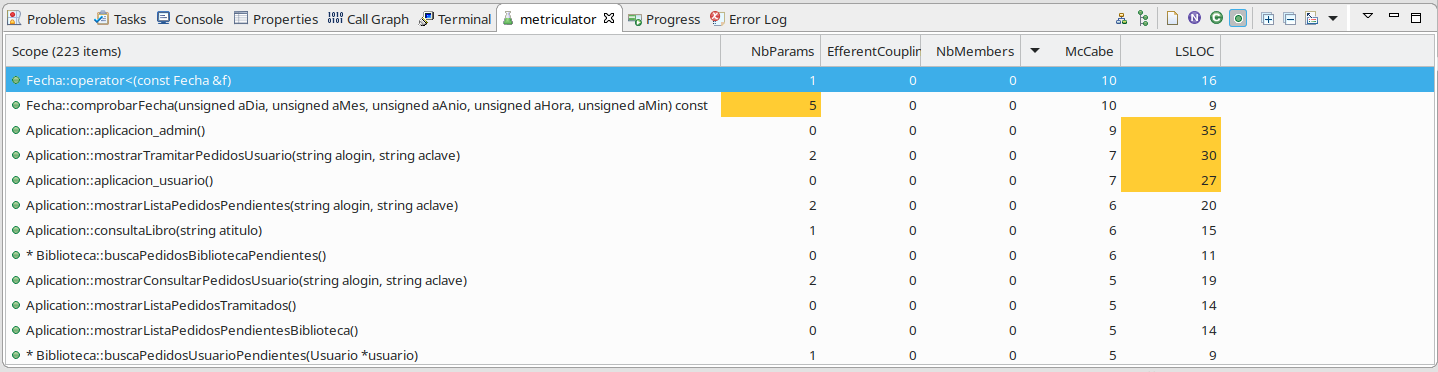
\includegraphics[scale=0.32]{img/captura111.png}
		\caption{Captura de pantalla de los resultados arrojados tras la ejecución de metriculator.}
		\label{captura111}
	\end{figure}

	\begin{figure}[H]
		\centering
		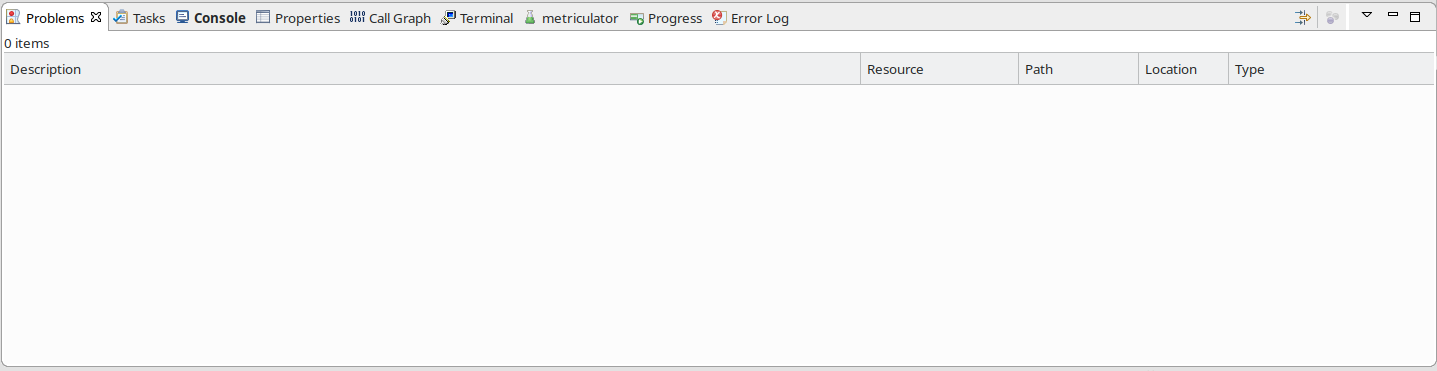
\includegraphics[scale=0.32]{img/captura112.png}
		\caption{Captura de pantalla de los resultados arrojados tras la ejecución de cppcheck.}
		\label{captura112}
	\end{figure}

	\paragraph{}Los resutados devueltos por metriculator están ordenados por el valor de McCabe, de mayor a menor, y se puede observar como no existe ningún módulo con un V(G)$>$10.
	
	\paragraph{}Tras ejecutar cpppcheck, este no nos devuelve ninguna incidencia.
	
	\paragraph{}Estos resultados nos permiten considerar como cumplidos satisfactoriamente los objetivos fijados para esta práctica.
	
\newpage